\section{Methodology}
\label{sec:Methodology}


\begin{figure*} [!t]
\begin{center}
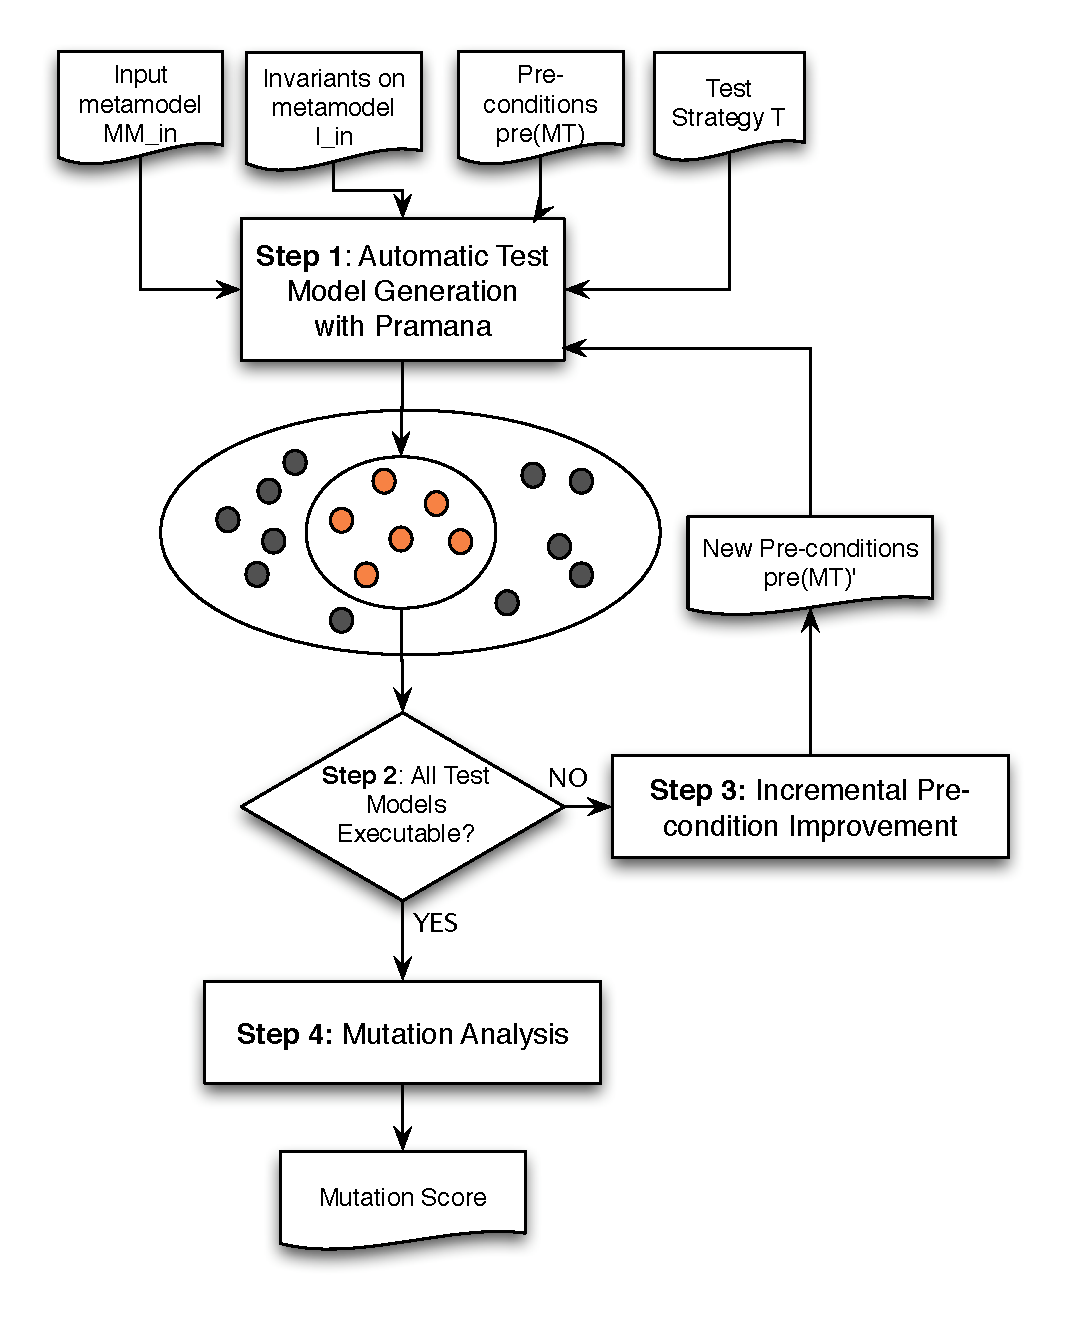
\includegraphics[height=5 in]{./figures/methodology.eps}
\end{center}
\caption{Methodology for Automatic Test Generation and Mutation Analysis}
\label{fig:methodology}
\end{figure*}

We outline the methodology for test generation  using {\Pramana} and empirical evaluation of the generated test models via mutation analysis in Figure \ref{fig:methodology}. The methodology uses  the foundational ideas we present in Section \ref{sec:Foundation} into a workflow. 

 Concisely, the test model generation workflow follows the steps:

\noindent \textbf{Step 1:} {\Pramana} transforms input metamodel $MM_{in}$, its invariants $I_{in}$, the transformation pre-condition $pre(MT)$ of transformation $MT$ and test strategy $T$ to an {\Alloy} model (details in Sections \ref{sec:sec:transfo2Alloy}, \ref{sec:sec:testStrategy}). {\Pramana} solves the {\Alloy} model to generate instances that are in the input domain of $MT$.

\noindent \textbf{Step 2:} 	We try to execute all test models generated by {\Pramana} as input to $MT$.

\noindent \textbf{Step 3:}   If all test models are not executable  in Step 2, then we incrementally create new pre-conditions for $MT$ called $pre(MT)'$. These pre-conditions are created from rejected test models. We describe incremental pre-condition improvement in Section \ref{sec:sec:precond}. We go to Step 1. Step 1 is executed using the a new source of constraints coming from $pre(MT)'$. 

\noindent \textbf{Step 4:} 	 If all test models are executable  in Step 2, we perform mutation analysis using the generated test models with respect to the model transformation $MT$. Mutation analysis is described in Section \ref{sec:sec:ma}.

\subsection{Incremental Pre-condition Improvement}
\label{sec:sec:precond}

The execution of a transformation helps us discover new pre-condition constraints $pre(MT)'$ for the transformation $MT$. In this sub-section we present the approach to systematically create new pre-conditions.

\begin{figure*} 
\begin{center}
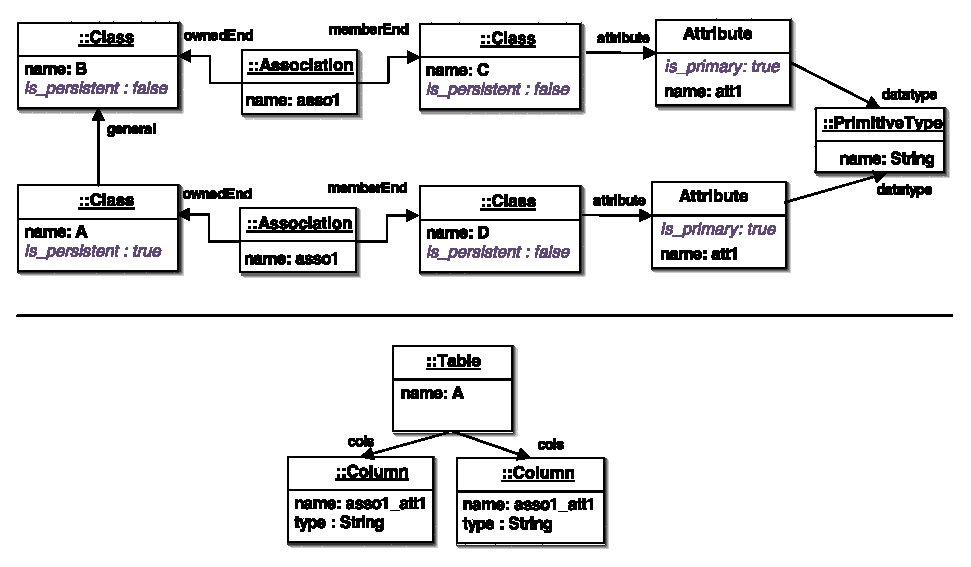
\includegraphics[width=6 in]{./figures/model-excerpt-for-constraint-improvment.eps}
\end{center}
\caption{Model Excerpt for Pre-condition Improvement}
\label{fig:modelExcerpt}
\end{figure*}

\noindent \textbf{Step 1:}  We execute the model transformation $MT$ with a test model $t$. 
\noindent \textbf{Step 2:}  The test model $t$ is rejected by the model transformation and the transformation terminates. The rejection of  a test model is often indicated by the raising of an exception by the transformation language. Some of the key sources for such rejections are:
					\begin{enumerate}
							\item \textbf{Insufficient memory} while creating modelling elements.
							\item \textbf{Infinite Loop} while navigating a test model.  For instance, this situation occurs when input models are navigated through a series of associations that can create loop structure in the transformation {\transfo}. These loops structures can navigation through diverse concepts such as  inheritance trees, associations, and type of attributes. The {\Kermeta} interpreter throws an  \textsf{StackOverflowError} exception when it detects such a problem. 
							\item \textbf{Transformation of an input model to an output model not in output domain}.  For instance, output models that do not satisfy the output meta-model specification and the post-condition $post(MT)$. In our case study, the transformation {\transfo} can produce ill-formed {\RDBMS} models. A typical example is when a table contains several columns with same name. We detect these inconsistencies by checking if output models conform to the output meta-model ({\ecore} model of the meta-model with invariants) and satisfy post-conditions of the model transformation. The Figure \ref{fig:modelExcerpt} illustrates this detection. It represents an excerpt (bottom part) of an output model produced by the original transformation of a generated (excerpt on the top part). 
					\end{enumerate}
					
\noindent \textbf{Step 3:}  We isolate inconsistent output models and corresponding test models. We then use a traceability mechanism and tool such as in \cite{glitia2008} to restrain the analysis of these models on excerpts such as the one illustrated in Figure \ref{fig:modelExcerpt}. Class named $A$ is transformed into one table because it is persistent. It redefined an association of the Class $B$. Two associations with the same name \emph{asso1} point  to classes with the same attribute/property \emph{att1}. Respecting the specification, the original transformations produces a table with two columns named \emph{asso1\_att1}. This does not conform to the {\RDBMS} meta-model and it is detected by our tool. Construction of such models can be prevented by generating objects with different names. 

\noindent \textbf{Step 4:}  We solve this inconsistency by creating a new pre-condition constraint that protects the transformation from executing such models. We also regenerate new models that satisfy the new pre-condition constraints. For instance, the faulty model excerpt in Figure \ref{fig:modelExcerpt} can help us produce a new pre-condition that states:

\emph{In the classes of an inheritance tree, two associations with the same name can't point to classes that have (or their parent) attributes with same names}.

Several new pre-conditions were discovered for the {\transfo} case study. We enlist nine newly discovered {\Alloy} facts in Appendix \ref{appendix:discoveredPrecondition} apart from the initial set of pre-condition constraints as shown in Appendix \ref{appendix:initialPrecondition}. These {\Alloy} facts can be easily expressed in {\OCL} to improve the pre-condition specification of {\transfo}. The conditions may even be applicable to commercial implementations of {\transfo}.

